We now introduce another approach based on the Edgeworth series to create accurate density approximations that avoids some of the issues of the Edgeworth series that we have demonstrated in the previous section.

We now introduce the idea of \textit{exponential tilting}. Consider a random random variable $X \sim \Rp$ with cumulant generative function $K$ and density $f$. We introduce the exponential family $\mathcal{T}_P = \{ P_\gamma \}_{\gamma \in \Rp}$ where each $P_\gamma \in \mathcal{T}_P$ is characterized by its density function $f_\gamma$ given by
\begin{equation*}
    f_\gamma(x) = f(x)\expf{\gamma^\top x - K(\gamma)}.
\end{equation*}
Note that by the definition of the cumulant generating function, $K(\gamma)$ is the right normalization factor for $f_\gamma$ and hence $f_\gamma$ integrates to 1 and is a valid density function. Furthermore, the original distribution $P$ is an element of $\mathcal{T}_P$ with $P = P_0$. Given two distributions in $\mathcal{T}_P$, their densities only differ by the ratio of $\expf{\gamma^\top x - K(\gamma)}$. Since the following holds for any $\gamma \in \Rp$
\begin{equation} \label{eq-saddlepoint-original}
    f(x) = f_\gamma(x)\expf{K(\gamma) - \gamma^\top x},
\end{equation}
we can construct an approximation of $f$ by choosing $\gamma$ such that $f_\gamma$ can be accurately approximated.

Let us now consider a distribution $P$ with cumulant generating function $K$. We wish to use the previous argumentation to approximate the density $f$ of the mean $S$ of $n$ i.i.d.\,random variables distributed according to $P$. The cumulant generating function of $S$ in Equation (\ref{eq-saddlepoint-original}), we get
\begin{equation*}
    f(s) = f_\gamma(s)\expf{nK(\gamma / n) - \gamma^\top s}.
\end{equation*}
We can now get back to the question of the choice of $\gamma$. We are interested in choosing $\gamma$ such that the Edgeworth approximation of $\bar f_\gamma(x)$ is accurate. As seen in Remark \ref{rem-edge-mean}, the second order Edgeworth approximation of odd order gains half an order of accuracy when evaluated at the mean of the distribution. Since $\gamma$ can be chosen freely and differently for each value $s$ at which the density $f(s)$ is evaluated, we can choose $\gamma$ such that $s$ is the mean of the distribution $P_\gamma$. Given $\gamma \in \Rp$, the cumulant generating function of $P_\gamma$ is equal to
\begin{equation*}
    K_\gamma(t) = n\left[K((\gamma + t)/n) - K(\gamma/n)\right].
\end{equation*}
One sees that derivatives of the cumulant generating function $K_\gamma$ can be expressed in terms of the cumulant generating function $K$ by
\begin{equation} \label{eq-deriv-Kgamma}
    K_\gamma^s(t) = n^{1 - k} K((\gamma + t) / n),
\end{equation}
for any $s \in S(k)$. Thus, using a well-known property of exponential families, the expectated value of the distribution $P_\gamma$ can be expressed in terms of the gradient of the cumulant generating function of $X$,
\begin{equation*}
    \expec{S \sim P_\gamma}{S} = K'(\gamma / n).
\end{equation*}
For any $s \in \Rp$, we can now find a distribution $P_{\hat\gamma_s} \in \mathcal{T}_P$ with mean $s$ by solving
\begin{equation} \label{eq-saddlepoint}
    K'(\hat\gamma_s / n) = s.
\end{equation}
We choose to call the solution of this equation $\hat\gamma_s$ to emphasize the fact that instead of choosing one unique $\gamma$ and then construct an approximation of the density of $P_\gamma$ over $\Rp$, we find a different $\hat\gamma_s$ at each $s \in \Rp$ such that the Edgeworth approximation of the density of $P_{\hat\gamma_s}$ is accurate in $s$. Note that if $\hat\gamma_s$ solves (\ref{eq-saddlepoint}), it is also the maximum likelihood estimator of $\gamma$ within the model $\mathcal{T}_P$. We can then construct the Edgeworth approximation $e_k(s; \kappa(\hat\gamma_s))$ to the density $f_{\hat\gamma_s}$ with
\begin{equation*}
    f_{\hat\gamma_s}(s) = e_k(s; \kappa(\hat\gamma_s)) + o(n^{(1-k)/2}).
\end{equation*}
Replacing this in the expression of $f$ in terms of $f_{\hat\gamma_s}$ gives
\begin{align}
    f(s) &= \expf{nK(\hat\gamma_s / n) - \hat\gamma_s^\top s}\left[e_k(s; \kappa(\hat\gamma_s)) + o(n^{(1-k)/2})\right]\nonumber\\
    &= g_k(s; K)\left[1 + o(n^{(1-k)/2})\right]. \label{eq-saddle-exp}
\end{align}
A special case of particular interest is for $k = 3$. In this case, the Edgeworth approximation of $P_{\hat\gamma_s}$ is equal to its normal approximation and is given by
\begin{equation*}
    e_3(s; \kappa(\hat\gamma_s)) = (2\pi)^{-p/2}|\Sigma_{\hat\gamma_s}|^{-1/2}\expf{-\frac{1}{2}(s - \mu_{\hat\gamma_s})^\top \Sigma_{\hat\gamma_s}^{-1/2}(s - \mu_{\hat\gamma_s}) },
\end{equation*}
where $\mu_{\hat\gamma_s}$ and $\Sigma_{\hat\gamma_s}$ are the mean and covariance of $P_{\hat\gamma_s}$. By the choice of $\hat\gamma_s$, we have that $\mu_{\hat\gamma_s} = s$ and hence the term in the exponential is equal to zero. Furthermore, the covariance matrix $\Sigma_{\hat\gamma_s}$ is equal to $K_{\hat\gamma_s}''(\hat\gamma_s)$, the Hessian of $K_{\hat\gamma_s}$ evaluated at $\hat\gamma_s$. From Equation (\ref{eq-deriv-Kgamma}), $K''_{\hat\gamma_s}(\hat\gamma_s) = n^{-1} K''(\hat\gamma_s/n)$ and we get 
\begin{equation} \label{eq-saddle-3}
    g_3(s; K) = \left(\frac{n}{2\pi}\right)^{p/2}|K''(\hat\gamma_s/n)|^{-1/2} \expf{nK(\hat\gamma_s / n) - \hat\gamma_s^\top s}.
\end{equation}
We call this approximation the \textit{Saddlepoint approximation}. We can see that the Saddlepoint approximation is always positive, and by Remark \ref{rem-hermite-odd} and the choice of $\hat\gamma_s$,
\begin{align}
    f(s) 
    &= g_3(s; K)(1 + o(n^{-1}))\nonumber\\
    &= g_3(s; K)\left[1 + \frac{b(\hat\gamma_s / n)}{2n} + o(n^{-2})\right], \label{eq-saddle-o2}
\end{align}
where $b(\hat\gamma_s / n)$ is the coefficient of the terms of order $O(n^{-1})$ in the Edgeworth expansion of the tilted density. We justify this expansion error in the following theorem.

\begin{theorem}
    Let $P$ be a distribution with cumulant genrating function $K$ and $k \in \N_{\geq 2}$ such that all cumulants of $P$ of order up to $k$ exist. Suppose that for every $s \in \Rp$, Equation (\ref{eq-saddlepoint}) has a unique solution $\hat\gamma_s \in U$. Let $n \in \N$ and $X_1, \ldots, X_n \simiid P$ and $S$ be the mean
    \begin{equation*}
        S = n^{-1} \sum_{i=1}^n X_i.
    \end{equation*}
    Then, if the density $f_S$ of $S$ exists, the approximation $g_k(\cdot; K)$ given in Equation (\ref{eq-saddle-exp}) approximates $f_S$ pointwise with an relative error of order $o(n^{\ceil{(1-k)/2)}})$.
\end{theorem}
\begin{proof}
    This result is a direct consequence of Theorem \ref{thm-edgeworth} applied pointwise to the tilted distribution $P_{\hat\gamma_s}$ for every $s \in \Rp$. As discussed above, the Remark \ref{rem-hermite-odd} implies that only powers of $n^{-1}$ have non-vanishing coefficients in the Edgeworth approximation of the tilted densities, which in turns implies that the Edgeworth approximation error in each point is of order $o(n^{\ceil{(1-k)/2)}})$.
\end{proof}

While the Saddlepoint approximation shows many advantages over the Edgeworth approximation, it is important to note that the Saddlepoint approximation uses information from the complete cumulant generating function of the approximated density. The Edgeworth approximation on the other hand only uses the first $k$ moments of the distributions, which are evaluations of derivatives of the cumulant generating function in 0. 

\begin{figure}[h]
    \textbf{Approximation error of $\Gamma(2,1)$ standardized sums with $n=10$}
    \centering
    \subfloat{
        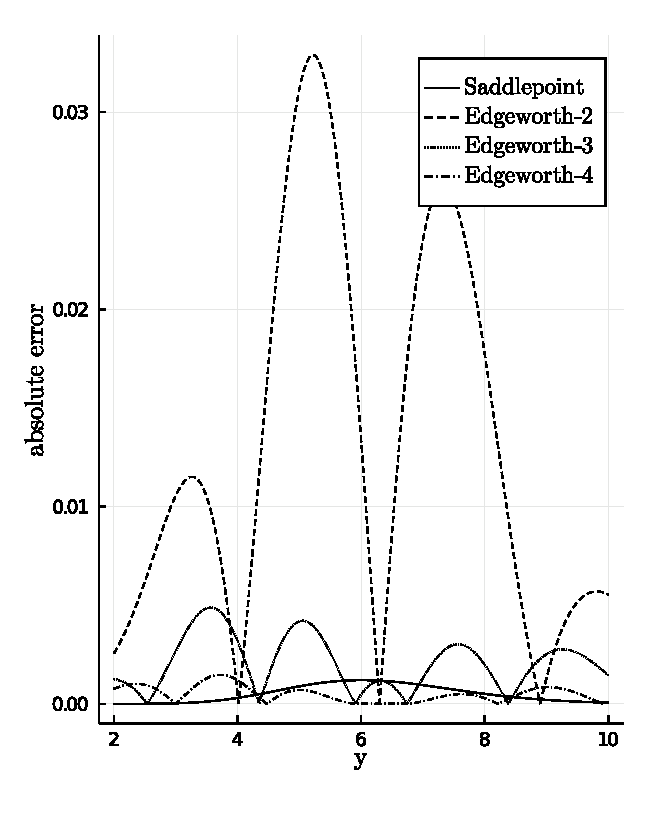
\includegraphics[width=8cm]{saddlepoint_and_edgeworth_err_abs_gamma21_10_terms.eps} 
    }
    \subfloat{
        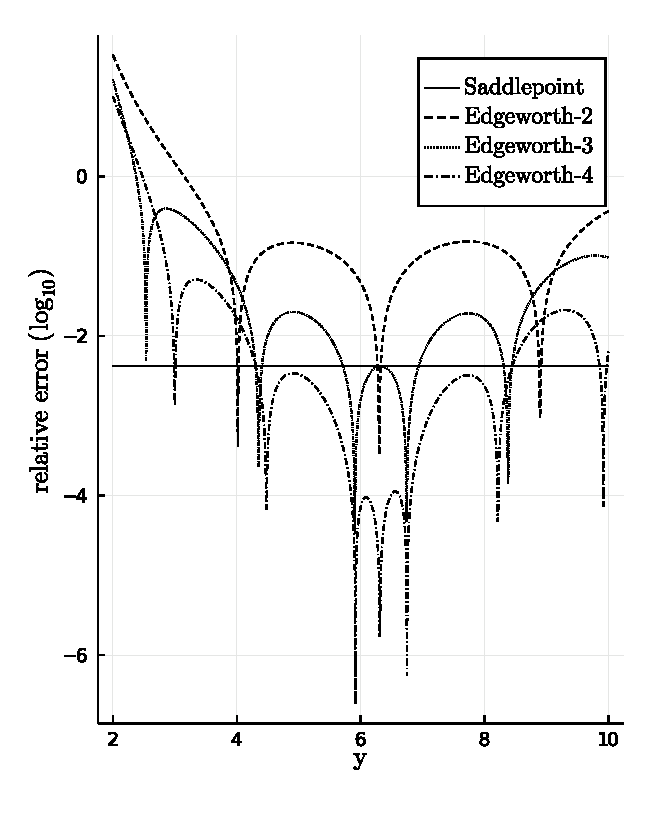
\includegraphics[width=8cm]{saddlepoint_and_edgeworth_err_rel_gamma21_10_terms.eps} 
    }
    \caption{Study of the approximation error of the Saddlepoint approximation on a standardized sum of $n=10$ of $\Gamma(2, 1)$ random variables. Both panel exposes properties studied of the Saddlepoint approximation: the accurate rellative error, the gain in order of approximation and the uniform relative error of the approximation for sums of Gamma random variables.}
    \label{fig-saddlepoint-err}
\end{figure}

\begin{example} \label{ex-gamma-saddle}
    Continuing Example \ref{ex-gamma-edge}, we can analyze the behaviour of the Saddlpoint approximation to the mean $Y = n^{-1}\sum_{i=1}^n X_i \in \R_+$ where $X_1, \ldots, X_n \simiid \Gamma(p, \lambda)$. The cumulant generating function of the $\Gamma(n, p)$ distribution is $K(t) = p\logf{\lambda} - p\logf{\lambda - t}$ and its first derivative is $K'(t) = p / (\lambda - t)$. For any $s \in \R_+$, the Saddlepoint $\hat\gamma_s$ is given by the solution to the Saddlepoint Equation (\ref{eq-saddlepoint}), which here becomes
    \begin{equation*}
        \frac{p}{\lambda - \hat\gamma_s/n} = s \Rightarrow \hat\gamma_s = n\left(\lambda - \frac{p}{s}\right).
    \end{equation*}
    In Figure \ref{fig-saddlepoint-err}, we demonstrate how the Saddlepoint approximation of order 3 compares to the Edgeworth approximation when approximating a standardized sum of $n$ random variables independently distributed according to $\Gamma(2, 1)$. Since the standardized sum can be obtained by multiplying the mean by a factor of $\sqrt{n}$, the Saddlepoint approximation is easily adapted by change of variable. Both panels show accurate approximation properties both in terms of relative and absolute error.
    
    In this example, it is also interesting to examine the concrete form of the Saddlepoint approximation $g_3$. Replacing the relevant quantities in Equation (\ref{eq-saddle-3}), we obtain that the Saddlepoint approximation is
    \begin{align*}
        g_3(s; K) &= \sqrt{\frac{n}{2\pi K''(\lambda - \frac{p}{s})}} \expf{nK\left(\lambda - \frac{p}{s}\right) - n\left(\lambda - \frac{p}{s}\right)s}\\
        &= \sqrt{\frac{n}{2\pi s^2/p}} \expf{n\left(p\logf{\lambda} - p\logf{p/s}\right) - ns\lambda + np}\\
        &= (n\lambda)^{np}s^{np-1}\expf{-sn\lambda} \times \frac{(np)^{1/2-np}\expf{np}}{\sqrt{2\pi}}.
    \end{align*}
    Consider now the Stirling's formula for the gamma function
    \begin{equation*}
        \Gamma(z) \approx \sqrt{2\pi}z^{z-1/2}\expf{-z}.
    \end{equation*}
    We recognize that the second term in the expression of $g_3(s; K)$ corresponds to the inverse of the Stirling's approximation to $\Gamma(np)$. The Saddlepoint approximation to the density of the mean of $\Gamma(p, \lambda)$ variables thus corresponds to the density of the true distribution $\Gamma(np, n\lambda)$ of the mean, where the gamma function has been replaced by the Stirling's approximation. This has the interesting consequence that the relative error of the Saddlepoint approximation does not depend on $s$, the point at which the density is evaluated, but rather only depends on $n$. This behaviour is also exposed in Figure \ref{fig-saddlepoint-err} where the relative error of the Saddlepoint approximation is a straight horizontal line. Daniels \cite{daniels1954saddlepoint} characterizes the class of distributions for which the uniform relative approximation error holds.
\end{example}

Consider now applying the Saddlepoint approximation to an exponential family $\mathcal{P} = \left\{P_\theta\right\}_{\theta}$ with natural parameter $\theta \in \Rp$. The density $f_\theta$ of $P_\theta \in \mathcal{P}$ is given by
\begin{equation*}
    f_\theta(x) = \expf{\theta^\top T(x) - \mathcal{H}(\theta) - \mathcal{G}(x)}.
\end{equation*}
Given a random sample $x = (x_1, \ldots, x_n)$ of $P_\theta$, the loglikelihood function is given by
\begin{equation*}
    \ell(\theta; x) = \theta^\top \sum_{i=1}^n T(x_i) - n \mathcal{H}(\theta) = n\left[\bar t - \mathcal{H}(\theta)\right],
\end{equation*}
where $\bar t$ is the sample average of the sufficient statistic, $\bar t = n^{-1}\sum_{i=1}^n T(x_i)$. Hence, the maximum likelihood estimator of $\theta$ is the value $\hat\theta_{\bar x} \in \Rp$ satisfying the score equation
\begin{equation} \label{eq-score-expfam}
    \mathcal{H}'(\hat\theta_{\bar t}) = \bar t.
\end{equation}
For simplicity, we will assume that $\mathcal{H}'$ is one-to-one to ensure that (\ref{eq-score-expfam}) has a unique solution $\hat\theta_{\bar t}$. In the exponential family $\mathcal{P}$, it can be shown that the cumulant generating function of any member $P_\theta \in \mathcal{P}$ is given by $K_\theta(t) = \mathcal{H}(\theta + t) - \mathcal{H}(\theta)$ and thus $K'_\theta(t) = \mathcal{H}'(\theta + t)$. Using the cumulant generating function in the score equation gives
\begin{equation*}
    K'_\theta(\hat\theta_{\bar t} - \theta) = \bar t.
\end{equation*}
Considering the Saddlepoint Equation given in (\ref{eq-saddlepoint}), we notice that the  parameter $\hat\gamma_{\bar t}$ of the tilted family nearly correspounds to the maximum likelihood estimator $\hat\theta$ with
\begin{equation*}
    \hat\gamma_{\bar t}/n = \hat\theta_{\bar t} - \theta.
\end{equation*}
Using this in the first order Saddlepoint approximation (\ref{eq-saddle-3}), we obtain that the Saddlepoint approximation for the average $\bar T = n^{-1}\sum_{i=1}^n T(X_i)$, \note{maybe justify that $T(X)$ is also in exp fam with same cgf and param, which is why the rest works} where $X_1, \ldots, X_n \simiid P_\theta$, is
\begin{align*}
    g_3(\bar t; K_\theta) 
    &= \sqrt{n} (2\pi)^{-p/2}|K_\theta''(\hat\theta_{\bar t} - \theta)|^{-1/2} \expf{nK_\theta(\hat\theta_{\bar t} - \theta) - (\hat\theta_{\bar t} - \theta)^\top \bar t}\\
    &= \sqrt{n} (2\pi)^{-p/2}|\mathcal{H}''(\hat\theta_{\bar t})|^{-1/2} \expf{n(\mathcal{H}(\hat\theta) - \mathcal{H}(\theta_{\bar t})) - (\hat\theta_{\bar t} - \theta)^\top \bar t}\\
    &= \sqrt{n} (2\pi)^{-p/2}|j(\hat\theta_{\bar t})|^{-1/2} \expf{\ell(\theta; \bar t) - \ell(\hat\theta_{\bar t}; \bar t)},
\end{align*}
where we have used that $\mathcal{H}''(\hat\theta)$ is equal to the observed Fisher information $j(\hat\theta)$. Daniels \cite{daniels1958} notes that this approximation can further be used to approximate the distribution of the maximum likelihood estimator. Let $\hat\Theta$ be the random variable solving the score equation $\mathcal{H}'(\hat\Theta) = \bar T$, then, by change of variable, we can use the approximation above to construct an approximation $p^*$ to the distribution of $\hat\Theta$,
\begin{equation*}
    p^*(\hat\theta; \theta, \bar t) = \sqrt{n} (2\pi)^{-p/2}|j(\hat\theta)|^{-1/2} \expf{\ell(\theta; \bar t) - \ell(\hat\theta; \bar t)} \abs{\frac{\d \hat\theta}{\d \bar t}}^{-1}.
\end{equation*}
To compute the determinant of the Jacobian of the transformation $\hat\theta(\bar t)$, we can differentiate the score equation with respect to $\hat\theta$ to find $\mathcal{H}''(\hat\theta) = (\d \bar t / \d \hat\theta)$ and hence $(\d \hat\theta / \d \bar t) = \mathcal{H}''(\hat\theta)^{-1} = j(\hat\theta)^{-1}$, giving
\begin{equation} \label{eq-pstar}
    p^*(\hat\theta; \theta, \bar t) = \sqrt{n} (2\pi)^{-p/2}|j(\hat\theta)|^{1/2} \expf{\ell(\theta; \bar t) - \ell(\hat\theta; \bar t)}.
\end{equation}
While the dependence on $\bar t$ naturally comes from the proposed derivation of the $p^*$ approximation, it is often more convenient to parametrize the loglikelihood and $p^*$ approximations in terms of the maximum likelihood estimator $\hat\theta(\bar t)$. This is possible since we have assumed that the score equations (\ref{eq-score-expfam}) is uniquely solvable which implies that the maximum likelihood estimator $\hat\theta(\bar t)$ is sufficient \note{actually, prob. don't need uniqueness}. We will then write
\begin{equation*}
    p^*(\hat\theta; \theta, \hat\theta) = \sqrt{n} (2\pi)^{-p/2}|j(\hat\theta)|^{1/2} \expf{\ell(\theta; \hat\theta) - \ell(\hat\theta; \hat\theta)}.
\end{equation*}
This also highlights the fact that the $p^*$ approximation inherited its locality from the Saddlepoint approximation, since the density $p^*(\hat\theta; \theta, \hat\theta)$ is different at each point $\hat\theta$ at which it is evaluated. The $p^*$ approximation can also be used in many different situation where the distribution of refence is not necessarily an exponential family. It has been derived and studied in a much broader generality by a series of articles and books by Barndorff-Nielsen \cite{BarndorffNielsen1980,BarndorffNielsen1983}.  

Suppose now that the exponential family $\mathcal{P}$ has an alternative parametrization $\{ P_\phi \}$ such that there exists a diffeomorphism $\phi = \phi(\theta)$ satisfying $\hat\phi = \phi(\hat\theta)$, where $\hat\phi$ and $\hat\theta$ are the maximum likelihood estimators in their respective parametrizations. Then, 
\begin{align*}
    p^*(\hat\phi; \phi, \hat \phi) 
&= \sqrt{n} (2\pi)^{-p/2}|j_\phi(\hat\phi)|^{1/2} \expf{\ell(\phi; \hat \phi) - \ell(\hat\phi; \hat \phi)}\\
&= \sqrt{n} (2\pi)^{-p/2}\left(|j_\theta(\theta(\hat\phi))|\abs{\frac{\d \hat\theta}{\d \hat\phi}}^{-2}\right)^{1/2} \expf{\ell(\theta(\phi); \theta(\hat \phi)) - \ell(\theta(\hat\phi); \theta(\hat \phi))}\\
&= p^*(\theta(\hat\phi); \theta(\phi), \theta(\hat \phi))\abs{\frac{\d \hat\theta}{\d \hat\phi}}^{-1}.
\end{align*}
Hence, the $p^*$ approximation is \textit{invariant under reparametrization}. 

\begin{example}
    Consider now estimating the density of the maximum likelihood estimator of the parameter $\lambda \in \R_+$ of an exponential distribution. The density of the distribution $\text{Exp}(\lambda)$ is
    \begin{equation*}
        f_\lambda(x) = \lambda \expf{-\lambda x}.
    \end{equation*}
    To make direct use of the $p^*$ approximation in Equation (\ref{eq-pstar}), we must work in the natural parametrization of the exponential distribution. For $\lambda \in R_+$, the corresponding natural parameter is $\theta = -\lambda \in \R_-$ and the density of $\text{Exp}(\theta)$ is then $f_\theta(x) = \expf{ \theta x + \logf{-\theta}}$. Given a i.i.d.\,sample $x_1, \ldots, x_n$ of $\text{Exp}(\theta)$, we have the likelihood
    \begin{equation*}
        \ell(\theta; \bar x) = n\left[\theta \bar x + \logf{-\theta}\right],
    \end{equation*}
    where we used that the sufficient statistic is $T(x) = x$ and hence $\bar t = \bar x$ is the sample mean. The maximum likelihood estimator of $\theta$ is then $\hat\theta = -1/\bar x$ and the observed information is equal to $j(\theta) = 1/\theta^2$. The $p^*$ approximation to the density of $\hat\theta$ is then
    \begin{align*}
        p^*(\hat\theta; \theta, \hat\theta) 
        &= \sqrt{n} \frac{|\theta|^n}{|\hat\theta|^{n-1}}\expf{-n(\theta - \hat\theta)/\hat\theta} / \sqrt{2\pi}\\
        &= \sqrt{n} \frac{|\theta|^n}{|\hat\theta|^{n-1}}\expf{n\left[1 - \frac{\theta}{\hat\theta}\right]} / \sqrt{2\pi}
    \end{align*}
    Using the invariance of the $p^*$ approximation, we can obtain a $p^*$ approximation to the density of the maximum likelihood parameter $\hat\lambda$ in the original parametrization,
    \begin{equation*}
        p^*(\hat\lambda; \lambda, \hat\lambda) = p^*(\theta(\hat\lambda); \theta(\lambda), \theta(\hat\lambda)) \abs{\d \hat\theta / \d \hat\lambda}^{-1} = \sqrt{n} \frac{|\lambda|^n}{|\hat\lambda|^{n-1}}\expf{n\left[\frac{\lambda}{\hat\lambda} - 1\right]} / \sqrt{2\pi}.
    \end{equation*}
    Since $\text{Exp}(\lambda) = \Gamma(1, \lambda)$, the distribution of $\bar X$ is $\Gamma(n, n\lambda)$ and hence $\hat\lambda = \bar x$ is $\text{Inv-}\Gamma(n, n\lambda)$. We can compare the $p^*$ approximation to the commonly used Normal approximation to the distribution of the maximum likelihood estimator. In the exponential model, the Fisher information is $I(\lambda) = \lambda^{-2}$ and the following central limit theorem holds for the maximum likelihood estimator
    \begin{equation*}
        \sqrt{n}(\hat\lambda - \lambda) \xrightarrow[]{\d} N(0, I(\lambda)^{-1})\ \ \ \  \text{as } n \rightarrow \infty,
    \end{equation*}
    hence, $\hat\lambda$ is approximately $N(\lambda, \lambda^2/n)$ with an approximation error of the density of $o(n^{-1/2})$. In Figure \ref{fig-pstar-approx}, we compare these two approximations to the density of the MLE $\hat\lambda$ for $\lambda = 2$. As we can see in the left panel, the $p^*$ approximation properly fits the true density of $\hat\lambda$ and captures the bias of the $\hat\lambda$ estimator as opposed to the Normal approximation which is centered around the true value of $\lambda$. Furthermore, we can observe in the right panel how the relative error of the $p^*$ approximation is identical to the approximation error of the Saddlepoint approximation to the mean of $\Gamma(2, 1)$ seen in Example \ref{ex-gamma-saddle}. This is also a direct consequence of the invariance of the $p^*$ approximation since $\hat\Lambda$, the random variable associated to the MLE, is the inverse of the sample mean $\bar X$, which is a diffeomorphic transformation for positive reals.
    
    \begin{figure}
        \textbf{Error of $p^*$ approximation of MLE in $\textrm{Exp}(\lambda)$ model with $n=10$}
        \centering
        \subfloat{
            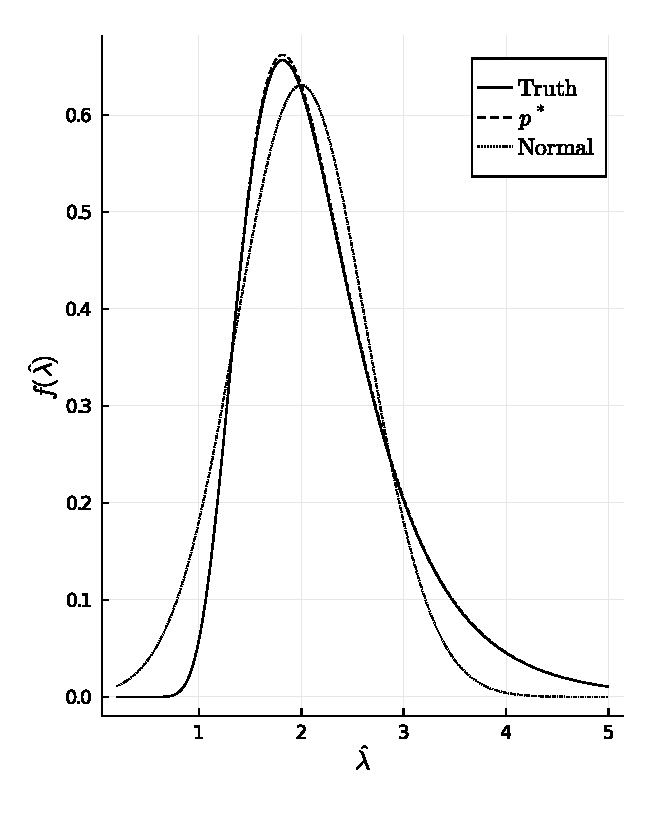
\includegraphics[width=8cm]{pstar_exp_dens.eps} 
        }
        \subfloat{
            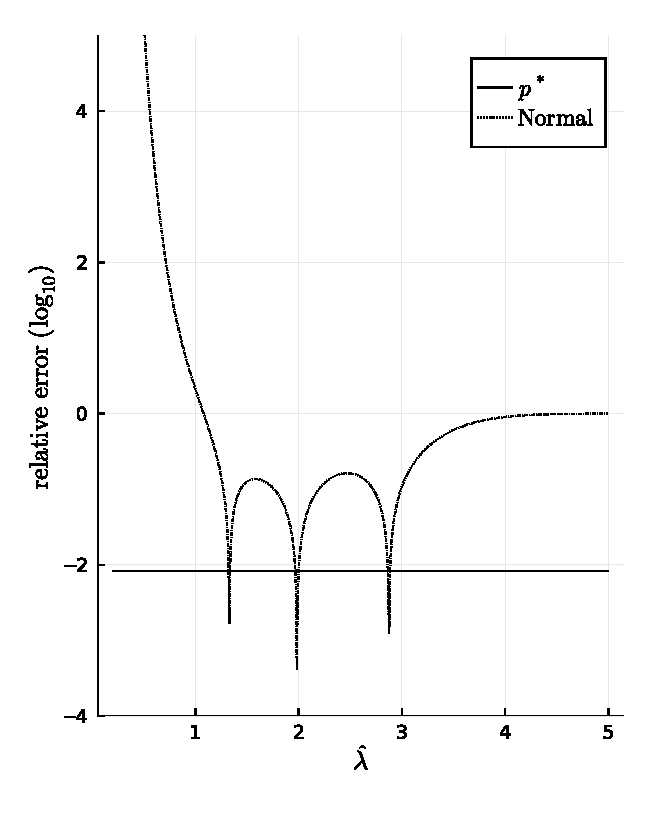
\includegraphics[width=8cm]{pstar_exp_err.eps} 
        }
        \caption{Study of the approximation error of the Saddlepoint approximation on a standardized sum of $n=10$ of $\Gamma(2, 1)$ random variables. Both panel exposes properties studied of the Saddlepoint approximation: the accurate rellative error, the gain in order of approximation and the uniform relative error of the approximation for sums of Gamma random variables.}
        \label{fig-pstar-approx}
    \end{figure}    

    \begin{lemma} \label{lem-char-integrable-convolution}
    The characteristic function $\xi$ of a random variable $X$ in $\Rp$ satisfies $\xi \in L^q(\Rp)$ for some $q > 1$ if and only if there exists a positive integer $l \in \N$ such that the density of a convolution of $l$ independent copies of $X$ exists and is bounded.
\end{lemma}
\begin{proof}
    This proof is an adaptation of the one-dimensional proof given in \cite[Lemma 2.4.4]{kolassa2006series}.

    The \textit{only if} direction is a direct consequence of Theorem \ref{thm-char-inversion}. Assuming that $\xi \in L^q(\Rp)$ we have that $\xi \in L^l(\Rp)$ for $l = \ceil{q}$ and hence,
    \begin{equation*}
        \intRp{t}{\abs{\xi(t)^l}} < \infty,
    \end{equation*}
    and so $\xi^l \in L^1(\Rp)$. Since $\xi^l$ is the characteristic function of a sum of $l$ independent copies of $X$, we can apply Theorem \ref{thm-char-inversion}, which gives us that the density of the convolution of $l$ copies of $X$ exists and is bounded.
    \newline
    We now prove the \textit{if} direction of the theorem. Assume that there exists a positive interger $j \in \N$ such that the density $f_j$ of a convolution of $j$ independent copies of $X$ exists and is bounded. Then, for any $r \in \R$,
    \begin{equation*}
        \int_{[-r, r]^p} \abs{\xi(t)}^{2j} \d t
        = \int_{[-r, r]^p} \abs{\xi(t)}^j\abs{\xi(t)}^j \d t
        = \int_{[-r, r]^p} \abs{\xi(t)}^j\abs{\xi(-t)}^j \d t,
    \end{equation*}
    where we use that $\abs{\xi(-t)} = \abs{\overline{\xi(t)}} = \abs{\xi(t)}$. Furthermore, by the definition of the characteristic function and using Fubini's theorem, we have that
    \begin{align*}
        \int_{[-r, r]^p} \abs{\xi(t)}^{2j} \d t
        &= \int_{[-r, r]^p} \left[\intRp{x}{f_j(x)\expf{it^\top x}}\right]\left[\intRp{y}{f_j(y)\expf{-it^\top y}}\right] \d t\\
        &= \intRp{x}{\intRp{y}{\int_{[-r, r]^p} f_j(x)f_j(y)\expf{it^\top (x - y)}\d t}}.
    \end{align*}
    Setting $z = y - x$ and using the identity $\sin x = (\expf{ix} - \expf{-ix}) / 2i$, we get
    \begin{align*}
        \int_{[-r, r]^p} \abs{\xi(t)}^{2j} \d t
        &= \intRp{x}{\intRp{z}{\int_{[-r, r]^p} f_j(x)f_j(x + z)\expf{-it^\top z}\d t}}\\
        &= \intRp{x}{\intRp{z}{f_j(x)f_j(x + z)\left[\prod_{k=1}^p \int_{[-r, r]}\expf{-it^\top z_k}\right]\d t}}\\
        &= \intRp{x}{\intRp{z}{f_j(x)f_j(x + z)\left[\prod_{k=1}^p \frac{\expf{-irz_k} - \expf{irz_k}}{-iz_k} \right]}}\\
        &= \intRp{x}{\intRp{z}{f_j(x)f_j(x + z)\left[\prod_{k=1}^p \frac{2 \sin(rz_k)}{z_k} \right]}}.
    \end{align*}
    Applying the change of variable $v = r z$ gives us
    \begin{align*}
        \int_{[-r, r]^p} \abs{\xi(t)}^{2j} \d t
        &= \intRp{x}{\intRp{v}{f_j(x)f_j(x + v/r)\left[\prod_{k=1}^p \frac{2 \sin(v_k)}{v_k/r} \right] r^{-p}}}\\
        &= \intRp{x}{\intRp{v}{f_j(x)f_j(x + v/r)\left[\prod_{k=1}^p \frac{2 \sin(v_k)}{v_k} \right]}}.
    \end{align*}
    Using the fact that $\sup_{x \in \R} \abs{\sin x / x} < 1$, we have that $\prod_{k=1}^p \frac{2 \sin(v_k)}{v_k} < 2^p$ and
    \begin{equation*}
        \int_{[-r, r]^p} \abs{\xi(t)}^{2j} \d t
        \leq \intRp{x}{f_j(x)\intRp{v}{f_j(x + v/r)}}
        = \intRp{x}{f_j(x)} = 1.
    \end{equation*}
    This shows that a finite upper bound on $\norm{\xi}_{2j}^{2j}$ that is independent of $r$ exists. This concludes the proof for $q = 2j$.
\end{proof}

    \subsection{Julia implementation of higher-order approximations}
One is often confronted with challenges when translating mathematical ideas into executable software. Edgeworth series in particular are simple in their mathematical definition, but hide the use of many mathematical concepts that, independently, are commonly cumbersome to translate into easy-to-use and bug-free software. A generic implementation of Edgeworth series requires the ability to compute derivatives, express and manipulate asymptotic expansions and combine those to create density approximations.

Luckily, modern programming languages and libraries allow to quickly develop algorithms that are both efficient and close to their mathematical counterpart. In this thesis, we make use of the Julia programming language \cite{bezanson2017julia} and Julia bindings to the computer algebra system SymPy \cite{sympy}. The Julia programming language was chosen because it allows to write code that is generic enough to be used in various scenarios and extended with the ecosystem of libraries. For instance, one basic block of the approximations developed in this thesis is the cumulant generating function of a distribution. The cumulant generating function of a $\Gamma(\alpha, \beta)$ distribution can be defined as the function
\begin{lstlisting}[language=Julia, mathescape, escapechar=\%]
julia> gamma(p, $\lambda$) = t -> p*log($\lambda$) - p*log($\lambda$-t)
\end{lstlisting}
This function can then both be used with concrete values of $p, \lambda$ and $t$, for instance $\textrm{gamma}(1.0, 2.0)(1.0) = 0.6931471805599453$. However, one can also define symbolic variables for $p$ and $\lambda$ to construct a symbolic expression of the cumulant generating function
\begin{lstlisting}[language=Julia, mathescape, escapechar=\%]
julia> @syms p::positive $\lambda$::positive
julia> gamma(p, $\lambda$)(t)
p*log($\lambda$) - p*log($\lambda$-1.0)
\end{lstlisting}
This modularity can be used to construct helper functions to manipulate cumulant generating functions based on other libraries. For instance, if we are interested in computing the cumulants of a distribution, we can use the same definition of the cumulant function together and use the TaylorSeries \cite{TaylorSeries} library to efficiently compute the derivatives of the cumulant generating function. This let's us define the following function to compute the first $n$ cumulants of a distribution from its cumulant generating function
\begin{lstlisting}[language=Julia, mathescape, escapechar=\%, basicstyle=\small]
function cumulants(K, n; T=Number)
    t = Taylor1(T, n+1)
    (K(t).coeffs ./ exp(t).coeffs)[2:end]
end
\end{lstlisting}
Julia's extensibility makes it easy to combine several libraries to develop more advanced functionalities. For instace, we can the code presented above to compute the generic formula of the mean and variance of a $\Gamma(p, \lambda)$ distribution without having to program the interaction between Julia's SymPy bindings and the TaylorSeries library
\begin{lstlisting}[language=Julia, mathescape, escapechar=\%]
julia> @syms p::positive $\lambda$::positive
julia> $\mu,\ \sigma^2$ = cumulants(gamma(p, $\lambda$), 2)
2-element Vector{Sym}:
   p/$\lambda$
   p/$\lambda^2$
\end{lstlisting}
We used the capability of Julia to compose high-level libraries in order to develop a generic procedures for manipulating cumulant generating functions and develop density approximations for sums and maximum likelihood estimators. As an example, Listing \ref{lst-edgeworth} implements an arbitrary-order Edgeworth expansion by combining the mathematical derivation of the Edgeworth series in Section \note{TODO add ref} and some of the ideas described above.

A particularly appealing example of the usage of the function in Listing \ref{lst-edgeworth} is to derive the generic formula of the Edgeworth series of a specific order given the required cumulants. We start by defining a function \lstinline{symcgf(cumulants)} which creates a cumulant generating function with cumulants provided as an argument. For instance,
\begin{lstlisting}[language=Julia, mathescape, escapechar=\%]
julia> @syms t::real $\kappa_3$::real $\kappa_4$::real
julia> K = symcgf([0.0; 1.0; $\kappa_3$; $\kappa_4$])
julia> cumulants(K, 5; T=Sym)
5-element Vector{Sym}:
 0
 1
 $\kappa_3$
 $\kappa_4$
 0
\end{lstlisting}
We can then use the \lstinline{edgeworth} from Listing \ref{lst-edgeworth} to compute the explicit formula for the Edgeworth series of order 4\footnote{To avoid writing out the Hermite polynomials, we use a sligthly modified version of the code in Listing \ref{lst-edgeworth} replacing Hermite polynomials by symbolic functions $H_k$.}
\newpage
\begin{lstlisting}[language=Julia, mathescape, escapechar=\%]
julia> edgeworth(K, n, 4; T=Sym)(x)
                                                    -$x^2$  
                  /                             \   ---
                  |    $\kappa_3^2$$H_6$(x)      $\kappa_4H_4$(x)      $\kappa_3H_3$(x)     |   2  
0.398942280401433 |1 + ------ + ------ + ------- | e    %\footnote{This output was lightly adapted to properly render in LaTeX. }%
                  |     72n       24n     6$\sqrt{n}$      |      
                  \                             /    

\end{lstlisting}
With $(2\pi)^{-1/2} \approx 0.398942280401433$, this formula corresponds expression derived in Equation (\ref{eq-edgeworth-1d-4}) of Example \ref{ex-edgeworth-1d}.

\begin{lstlisting}[language=Julia, mathescape, escapechar=\%, caption={Symbolic implementation of the Edgeworth expansion}, label={lst-edgeworth}, basicstyle=\small]
function edgeworth(K, nsum, order; T=Float64)
    H(k) = basis(ChebyshevHermite, k)
    finaltype = promote_rule(T, typeof(nsum))
    taylororder = 3*order+1

    # Define two symbolic variables t and n. We use t as
    # variable  of the cgf for computing Taylor series and
    # n as the symbolic number of elements in the sum in
    # order to be able to track terms of various orders of n.
    @vars t n::(positive, integer)

    # Start by constructing the cgf of $\sum (X_i - \mu)/\sqrt{\sigma^2 n}$,
    # as discussed in Remark %\ref{rem-centering}%.
    $\mu$, $\sigma^2$ = cumulants(K, 2; T=T)
    stdK = affine(K, -$\mu$, 1/sqrt($\sigma^2$*n))
    sumK = iidsum(stdK, n)

    # Use the new cgf to construct the expansion of the ratio 
    # of characteristic functions, as in Equation (%\ref{eq-char-expansion}%).
    ratio = exp(sumK(t) - t^2/2)
    expansion = ratio.series(t, n=taylororder).removeO()

    # Then proceed by truncating the expansion to the desired 
    # order and replace the symbolic n by its true value.
    expansion = collect(expand(expansion), n)
    expansion = truncate_order(expansion, n, (1-order)/2)
    expansion = subs(expand(expansion), n, nsum)

    # The `expansion` variable is now a symbolic polynomial 
    # in the variable t. We retrieve the density by Fourier 
    # inversion, by which we replace instances of t^k by the 
    # k-th Hermite polynomial as in Equation (%\ref{eq-edgeworth-full}%).
    $\alpha$star = collect(expansion, t).coeff.(t.^(0:taylororder))
    $\alpha$star = convert.(finaltype, $\alpha$star)
    polynomial = sum([$\alpha$star[i]*H(i-1) for i=1:length($\alpha$star)])

    # Finally, the approximate density can be constructed
    # as done in %\ref{eq-edgeworth-full}% and using Remark %\ref{rem-centering}%.
    function density(z)
        $\kappa_1$ = sqrt(nsum)*$\mu$; x = (z - $\kappa_1$) / sqrt($\sigma^2$)
        return exp(-x^2/2)/sqrt($\sigma^2$*2$\pi$) * polynomial(x)
    end
end
\end{lstlisting}

\end{example}
